\section{Muscle Visualization}
\label{sec:muscleVis}
In order to test, evaluate and later validate the proposed method, we started the development of a visualization software tool that is able to display geometry efficiently by using parallel hardware (GPU) techniques; the visualization software will also provide an interface to control simulation parameters.

%----------------------------------------------------------------------------------------

\subsection{Visualization Implementation}

By using a set of third party software tools, we assembled a rendering engine (Figure~\ref{fig:muscleVis}) that allows efficient display and control of a simulation that uses the proposed method. Open Source libraries for rendering, shading, graphical user interface, texture and geometry loading have been integrated to the visualization software; these tools are listed in Table~\ref{tab:thirdSw}.

\begin{figure}[!t]
	\centering
		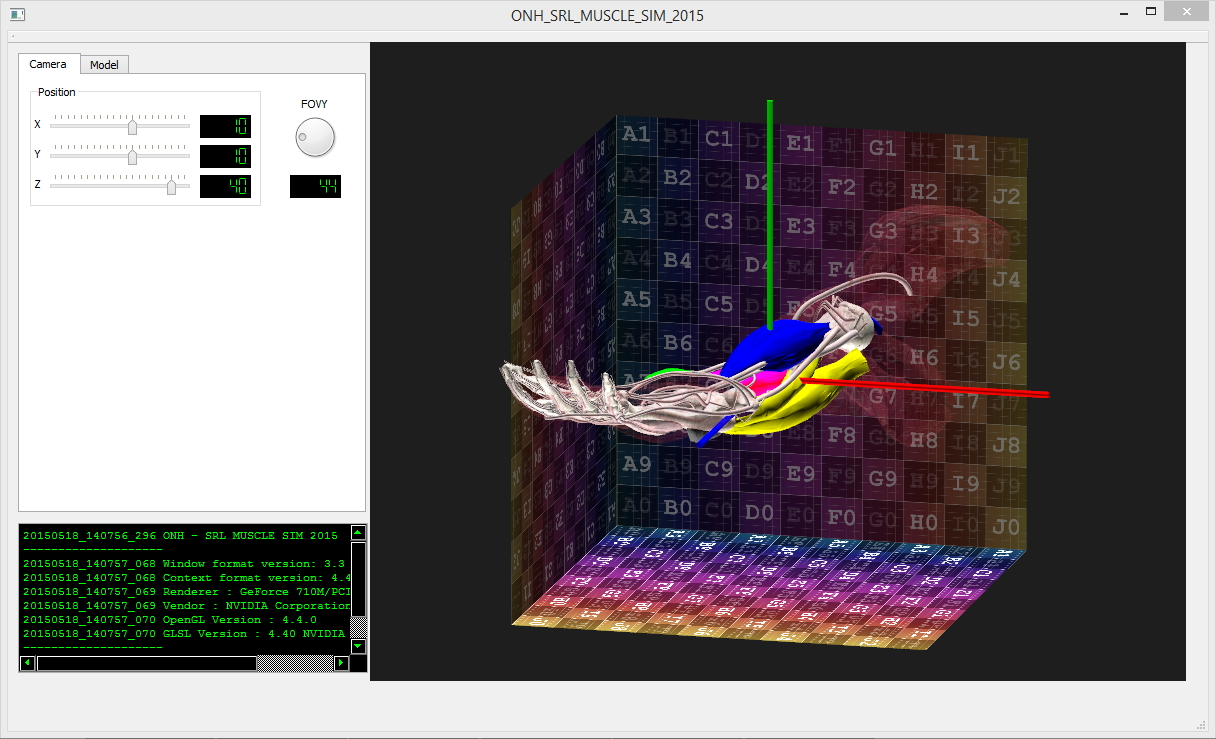
\includegraphics[width=0.8\textwidth]{./Figures/viewConfig.jpg}
	\caption[Muscle rendering.]{Muscle rendering tool.}
	\label{fig:muscleVis}
\end{figure}

\begin{table}[htbp]
  \centering
  \caption{Third party software for virtual muscle rendering}
    \begin{tabular}{rr}
    \toprule
    \multicolumn{2}{c}{\textbf{Third party software tools}} \\
    \midrule
    \textbf{Rendering Library} & OpenGL \\
    \textbf{Shading} & GLSL \\
    \textbf{GUI} & Qt 5.4.1 Community \\
    \textbf{Texture loader} & DevIL \\
    \textbf{Geometry loader} & ASSIMP \\
    \bottomrule
    \end{tabular}%
  \label{tab:thirdSw}%
\end{table}%

\subsection{Rendering Advances}

From the BodyParts3d~\citep{bodyParts3d} database, we have identified, colored and separated virtual muscle geometries (Figure~\ref{fig:muscleView}) of interest\textemdash right biceps brachii, brachialis, brachiordialis (Figure~\ref{fig:musclesFront}), pronator teres, triceps brachii, anconeus (Figure~\ref{fig:musclesBack})\textemdash that will serve as input for the muscle simulation. Together, all the arm meshes are composed of 271,004 faces which are rendered at interactive frame rates: up to 0.00588235 seconds per frame using a Nvidia GeForce 710M GPU as shown in Figure~\ref{fig:muscleRendering}, using transparent (Figure~\ref{fig:visFPS}) or opaque (Figure~\ref{fig:transparency}) geometry, thus allowing for simulation computations to be performed even on the same hardware.

\begin{figure}[t]
    \centering
    \begin{subfigure}[t]{0.45\textwidth}
        \centering
        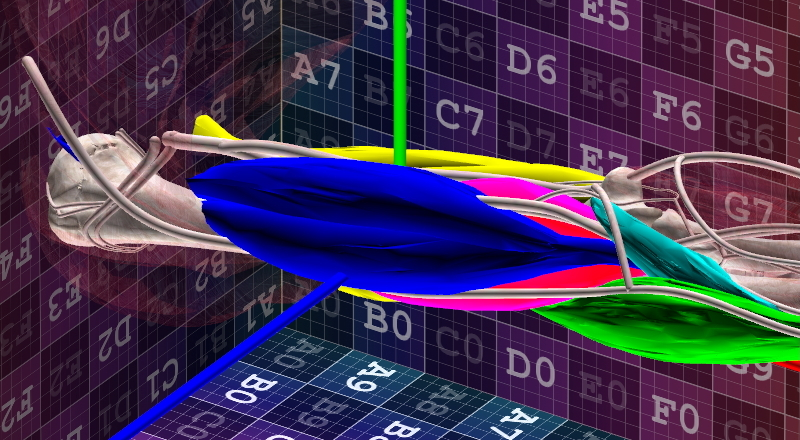
\includegraphics[width=\textwidth]{./Figures/musclesFront.jpg}
        \caption{Blue: biceps brachii. Purple: brachialis. Green: brachiordialis. Aqua: pronator teres.}
        \label{fig:musclesFront}
    \end{subfigure}
\hfill
    \begin{subfigure}[t]{0.45\textwidth}
        \centering
        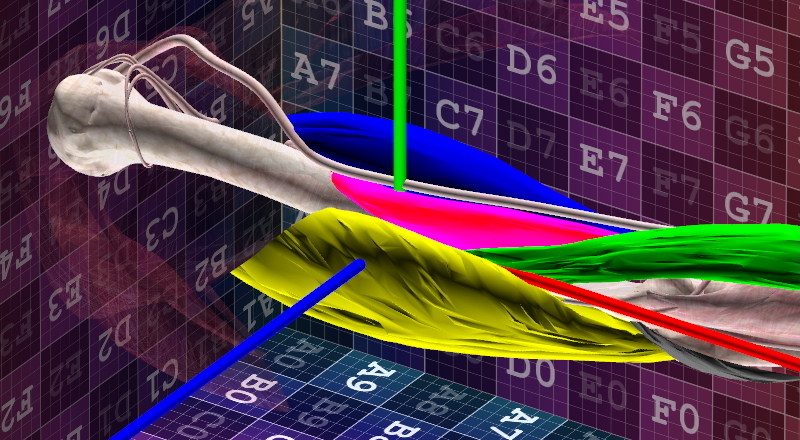
\includegraphics[width=\textwidth]{./Figures/musclesBack.jpg}
        \caption{Yellow: triceps brachii. Gray: anconeus.}
        \label{fig:musclesBack}
    \end{subfigure}

    \caption{Muscle geometry}
    \label{fig:muscleView}
\end{figure}

\afterpage{
\begin{figure}[t]
    \centering
    \begin{subfigure}[t]{0.45\textwidth}
        \centering
        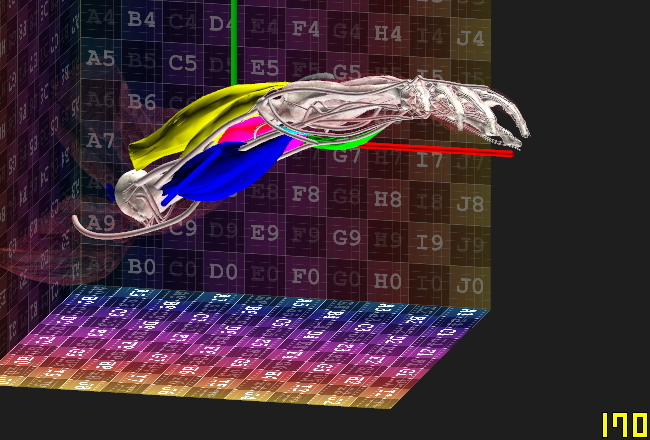
\includegraphics[width=\textwidth]{./Figures/visFPS.jpg}
        \caption{Interactive rate rendering.}
        \label{fig:visFPS}
    \end{subfigure}
	\hfill
    \begin{subfigure}[t]{0.45\textwidth}
        \centering
        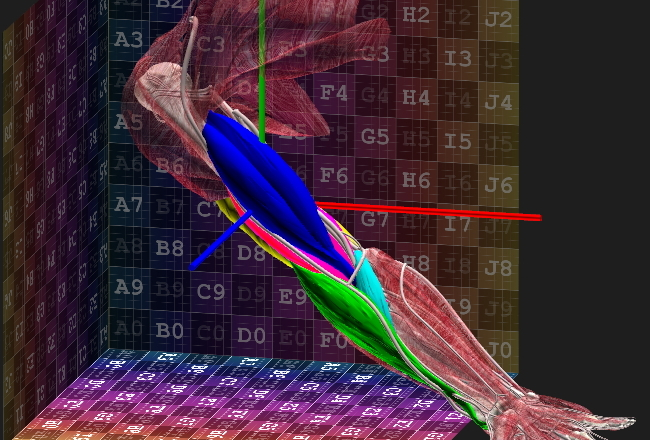
\includegraphics[width=\textwidth]{./Figures/transparencyConfig.jpg}
        \caption{Transparency control.}
        \label{fig:transparency}
    \end{subfigure}

    \caption{Muscle rendering}
    \label{fig:muscleRendering}
\end{figure}
}
%\begin{figure}
%    \centering
%    \begin{subfigure}[t]{0.45\textwidth}
%        \centering
%        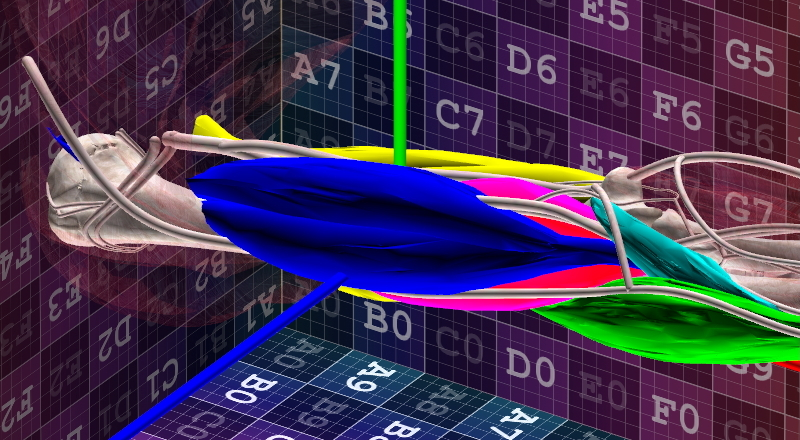
\includegraphics[width=\textwidth]{./Figures/musclesFront.jpg}
%        \caption{Blue: biceps brachii. Purple: brachialis. Green: brachiordialis. Aqua: pronator teres.}
%        \label{fig:musclesFront}
%    \end{subfigure}
%\hfill
%    \begin{subfigure}[t]{0.45\textwidth}
%        \centering
%        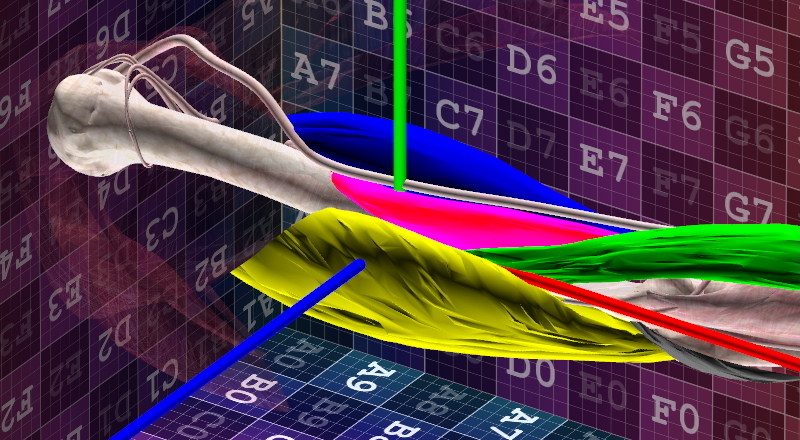
\includegraphics[width=\textwidth]{./Figures/musclesBack.jpg}
%        \caption{Yellow: triceps brachii. Gray: anconeus.}
%        \label{fig:musclesBack}
%    \end{subfigure}
%
%    \caption{Muscle geometry}
%    \label{fig:muscleView}
%\end{figure}
%
%
%\begin{figure}
%    \centering
%    \begin{subfigure}[t]{0.45\textwidth}
%        \centering
%        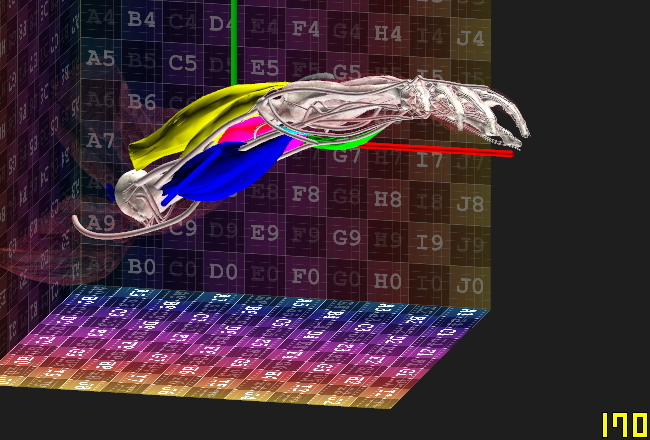
\includegraphics[width=\textwidth]{./Figures/visFPS.jpg}
%        \caption{Interactive rate rendering.}
%        \label{fig:visFPS}
%    \end{subfigure}
%	\hfill
%    \begin{subfigure}[t]{0.45\textwidth}
%        \centering
%        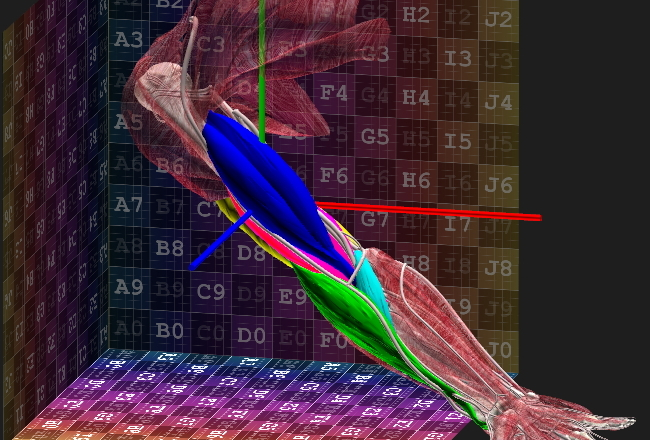
\includegraphics[width=\textwidth]{./Figures/transparencyConfig.jpg}
%        \caption{Transparency control.}
%        \label{fig:transparency}
%    \end{subfigure}
%
%    \caption{Muscle rendering}
%    \label{fig:muscleRendering}
%\end{figure}
